\chap{The Opportunity for Mobile Computing in the Dementia Epidemic} \label{chapter: lit-review}

\section{Introduction}
This chapter will explore the clinical presentation and prevalence of dementias, the challenges faced by sufferers and their carers, and the current efforts to treat and prevent the condition. It will then explore the opportunities for technology in these areas.

\section{Dementia}
Dementia is not a specific disease, but rather is a syndrome which describes a wide range of cognitive symptoms, caused by a number of conditions, which ultimately result in a progressive deterioration of cognitive functioning, beyond that of normal ageing. It affects thinking, memory, orientation, mental calculus, learning ability, language, and judgement. Along with the deterioration of cognitive function, motivation, social behaviour, and emotion control also deteriorate as the condition progresses.
As such dementia is a very personal and complex condition, causing a major impact in the quality of life of both those with the condition, and those who care for them.

\subsection{Prevalence}
As the average age of the population increases due to improvements in healthcare and lifestyle, dementia, and the number of people in its grip, is rising to meet it.
The prevalence of the condition is currently huge, with 47.5 million PwD globally. This number is projected to increase to 75.6 million by 2030, and by 2050 this number estimated to triple \cite{WHODementia2015}. People are living longer, and unfortunately age is still the greatest risk factor for dementias. The most common form of dementia is AD, which causes an estimated 60 to 80 percent of all cases \cite{2015AlzheimersDiseaseFactsFigures}. In relation to mortality, AD is the the 6th leading cause of total mortality in the United States \cite{NationalCenterforHealthStatistics2014}, and the 1st and 2nd leading cause of mortality of females and males over 80 years old, respectively, in the United Kingdom \cite{OfficeforNationalStatistics2014}.

\subsection{Treatment}
Unfortunately unlike other leading causes of mortality, such as heart disease and stroke \cite{WorldHealthOrganisation2015}, there are no current treatment options available to cure it or alter its course.
The search for a cure is a highly active research area, in which a number of new treatments are being investigated and are at various stages of clinical trials \cite{Burke2015}. There are also a number of therapeutic drugs that are used to maintain functioning, and to slow the rate of deterioration. The most common medications used for these purposes are cholinesterase inhibitors, which aid memory and judgement functioning. As of 2015, in the UK, the average number of prescriptions per person, for the general population, is 19.2 \cite{TheAssociationoftheBritishPharmaceuticalIndustry}. As such the task of medication management for PwD is an additional compounding issue.

\subsection{Causes}
Dementia is caused by a variety of diseases and injuries that cause actual physical changes in the brain. There is a general misunderstanding of dementia and its causes by the general public, which results in stigmatisation of the condition and creates barriers for those seeking diagnosis and care \cite{WHODementia2015}.
Each cause of dementia presents with similar symptoms, however, the pathology, prevalence, and the order and progression of symptoms vary. The most commonly occurring are discussed in the following Sections.

\textbf{Alzheimer's Disease.}
AD is the most common type of dementia, causing an estimated 60 to 80 percent of all cases \cite{2015AlzheimersDiseaseFactsFigures}.
Early symptoms of the disease include difficulty remembering names or recent events and conversations, apathy and depression. Later symptoms include disorientation and confusion, noticeably impaired communication, poor judgment and ultimately difficulty speaking, swallowing and walking.
It is generally accepted that AD is a slowly progressive brain disease, whose development occurs well before symptoms emerge, and in some cases, decades before \cite{DelaTorre2012, 2015AlzheimersDiseaseFactsFigures}.

\textbf{Vascular dementia.}
Vascular dementia (VD) accounts for approximately 10 percent of all dementia cases. Its prevalence increases with age, and is very common in older PwD, with approximately 50 percent having evidence of infarctions (death of tissue caused by a local lack of oxygen). In most cases VD coexists with AD \cite{2015AlzheimersDiseaseFactsFigures}.
Symptoms present slightly differently in VD, with impaired decision making, judgement and difficulty planning presenting first. The reasons behind VD are cardiovascular, resulting from blood vessel blockage and damage that leads to strokes and bleeding in the brain.

\textbf{Dementia with Lewy bodies.}
Lewy bodies are abnormal collections of the protein alpha-synuclein that accumulate in neurones. When these collections accumulate in the cortex, dementia can result. People with Dementia with Lewy bodies (DLB) can have a number of shared symptoms with AD, but their initial presentation will usually show sleep disturbances, visual hallucinations, and imbalances and slowness in gait. These symptoms can appear without significant memory issues, however, as with VD persons with DLB typically have coexisting AD.

\textbf{Mixed Dementia.}
Mixed dementia is identified as more than one cause of dementia. The prevalence of mixed dementia is now much more common that was previously believed, with approximately 50\% of those living with dementia having evidence of more than one cause. Within mixed dementias, the most common combinations are AD combined with VD, followed by AD and DLB, and then AD, DLB and VD combined.

\textbf{Others.}
There are a number of other causes for dementia, which are relatively uncommon, and are caused by gene defects, brain disorders, and mineral deficiencies. These include Parkinson's disease, Frontotemporal dementia, Creutzfeldt-Jakob disease, Hydrocephalus, Huntington's Disease, and Wernicke-Korsakoff Syndrome.

\subsection{Symptoms}
Dementia, irrespective of the cause, presents with a number of characteristic symptoms \cite{NationalHealthService2015} which  can be categorised as cognitive and psychological changes, as performed by the \citeauthor{MayoFoundationforMedicalEducationandResearch2015} \cite{MayoFoundationforMedicalEducationandResearch2015}:

\subsubsection{Cognitive changes}
\begin{itemize}[noitemsep,topsep=0pt]
\item Memory loss
\item Difficulty communicating or finding words
\item Difficulty with complex tasks
\item Difficulty with planning and organising
\item Difficulty with coordination and motor functions
\item Problems with disorientation, such as getting lost
\end{itemize}

\subsubsection{Psychological changes}

\begin{itemize}[noitemsep,topsep=0pt]
\item Personality changes
\item Inability to reason
\item Inappropriate behaviour
\item Paranoia
\item Agitation
\item Hallucinations
\end{itemize}

\subsection{Monitoring Progression}
The forms of dementia detailed earlier, AD, VD and DLB, are all progressive. Over time the underlying chemistry and structure of the brain suffer increasing damage. Each underlying cause has in influence on how the dementia progresses. For example AD, on average, has the slowest rate of progression, and loss of cognitive functioning is relatively linear. With VD, however, each stroke or mini-stroke causes a sudden drastic change in symptoms, often referred to as a step-wise progression.
The speed at which each PwD deteriorates varies widely from individual to individual, however, a number of factors have been identified as influencing the rate of progression:

\begin{itemize}[noitemsep,topsep=0pt]
\item Age - People who develop symptoms of dementia before 65 years, have a typically faster progression.
\item Genes - Family history or mutation
\item Overall Physical Health - Weak cardiovascular health, heart conditions, history and stroke, and diabetes, all have high probability of faster deterioration.
\end{itemize}

As dementia worsens, the PwD's ability to perform daily tasks becomes increasingly diminished. Eventually, the person will require support with daily living. It is therefore important to monitor and classify the progression of each persons symptoms.

\subsection{Assessment and Stages}
Health professionals use a battery of tests and scales to measure changes in cognitive functioning. The most common test to assess mental ability is the Mini Mental State Exam (MMSE) \cite{Folstein1975}, of which there are a number of variants e.g. e.g. the Modified Mini-Mental State Examination (3MS-R)\cite{Tschanz2002}, developed to improve the sensitivity and specificity of the assessments. Often an additional assessment of quality of life is performed, including an assessment of daily living skills, behaviour and overall functioning. Health professionals often refer to a PwD's symptoms and current state as being in one of 3 stages: Early, Middle, and Late \cite{2015AlzheimersDiseaseFactsFigures, AlzheimersAssociation2015a, Grout2015}.

\subsubsection{Early Stage}
The early stages begin with slight changes in a person's abilities or behaviours. Often, signs of change are mistaken in older people as a normal process of ageing, or in younger people as a result of stress or bereavement. Often these changes are missed, and are only recognised retrospectively, post diagnosis \cite{Grout2015}. A common early symptom is loss of short term memory, often resulting in the PWD having difficulty recalling details of recent events or difficulty learning new information.

Common symptoms for PwDs in early stages include:

\begin{itemize}[noitemsep,topsep=0pt]
\item forget recent conversations or events
\item misplacement of items in the home
\item difficulty finding the correct word
\item lose concentration or topic of conversation
\item slower at understanding new concepts
\item unwilling to adopt new processes
\item lose track of time and date
\item become poorer at making decisions or future planning
\item loss of interest in activities or people
\end{itemize}

During the early stages, it is common for the individual to become irritable, anxious or depressed. This can be due to distress due to the failure to complete certain tasks, such as those highlighted earlier.

\subsubsection{Middle Stage}
The middle stages of dementia bring a more marked change in symptoms and behaviours. The PwD will need increasing support for daily tasks, and may need frequent reminders to perform tasks, needing assistance to eat, get dressed, and maintain basic personal hygiene. Memory becomes markedly affected, resulting in increased forgetfulness and difficulty conversing in the short term, requiring sentences or questions to be repeated. Agnosia can also occur, resulting in the inability to recognise people, often confusing them for others. Due to increased forgetfulness and confusion, they put themselves and others at risk e.g. forgetting to take medications, or leaving the cooker on \cite{Grout2015}.
Changes in behaviour are most common during the middle stage, which can be challenging for their carers. Changes in emotional state may also occur, with PwD becoming upset easily, angry or aggressive. Again, this may be due to frustrations with their condition, or misinterpretations of their situation.

Other symptoms typically experienced during the middle stage include:
\begin{itemize}[noitemsep,topsep=0pt]
\item wandering due to confusion about their location
\item skewed day-night cycle (getting up at night, sleeping during day)
\item unknowingly behaving inappropriately
\item development of delusions, or less commonly, hallucinations
\end{itemize}


\subsubsection{Late Stage}
In the late stage the PwD will gradually become totally dependent on the care of others. Memory loss is very pronounced, with agnosia now affecting the recognition of those closest to them, as well as objects and their surroundings. Although agnosia now affects most sensations, causing poor understanding of speech, the PwD may have a response to affection, calm conversation, the sound of music, scents or stroking a pet \cite{Grout2015}.
Physically, the PwD may become weaker, have a shuffling gait, or require a wheelchair. Eventually they may become bed bound. In the late stages, the PwD may becoming increasingly restless, distressed and aggressive. This may also be due to a pain experienced by the PwD, which cannot be expressed verbally.

Other symptoms may include:
\begin{itemize}[noitemsep,topsep=0pt]
\item loss of speech
\item difficulty swallowing and eating
\item weight loss due to lack of food intake
\item incontinence
\end{itemize}

\subsection{Life Expectancy}
Those with AD typically live for 8 - 10 years after symptoms emerge. This figure varies widely depending on the age of the person, and if there are additional compounding factors and conditions \cite{Grout2015}.

\subsection{Risk Factors}
As with any health condition, there are a number of risk factors associated with it. The factors can be categorised as genetic, environmental and lifestyle \cite{Deckers2015, Norton2015-TRCI}.

\subsubsection{Genetic Risk Factors}
\textbf{Family history.}
Family history can play a role in the risk of developing dementia, particularly within AD. Those with a first degree relative, such as parent, brother, sister, or child with AD have a much greater risk of developing dementia. The risk also increases if more than one family member has the illness \cite{AlzheimersAssociation2015b}.

\textbf{Genetic Mutations.}
There are number of specific genetic mutations that place an individual at a significantly greater risk of developing dementia. There are clinical tests that can be performed to detect these mutations \cite{MayoFoundationforMedicalEducationandResearch2015a}.

\textbf{Down syndrome.}
It is common for those with Down syndrome to develop the plaques and tanges associated with AD, resulting in dementia in middle age.

\subsubsection{Environmental Risk Factors}

\textbf{Age.}
As age increases so does the risk of all forms of dementia, especially after 65 years. It must be noted that dementia is not a normal part of ageing, and should not be considered so.

\textbf{Education level.}
A low education level has been linked in the onset of AD. Having a higher level of education does reduce the risk of developing AD, but has no effect on the rate of progression once acquired \cite{Wilson2009}.
The reasons for this are unclear, however, many researchers advocate the ``cognitive reserve'' hypothesis \cite{Stern2012}; suggesting that someone who has spent a lifetime carrying out mentally stimulating activities will develop a larger capacity to deal with the natural atrophy in the brain in older age, and also stave off damage caused by dementias \cite{Norman2007, AlzheimerEurope2015}. A visual representation of how memory function is predicted to change in those with low and high cognitive reserves is presented in Figure \ref{fig: lancet-neurology-adpathology} \cite{Stern2012}.

\begin{figure}[h]
    \centering
    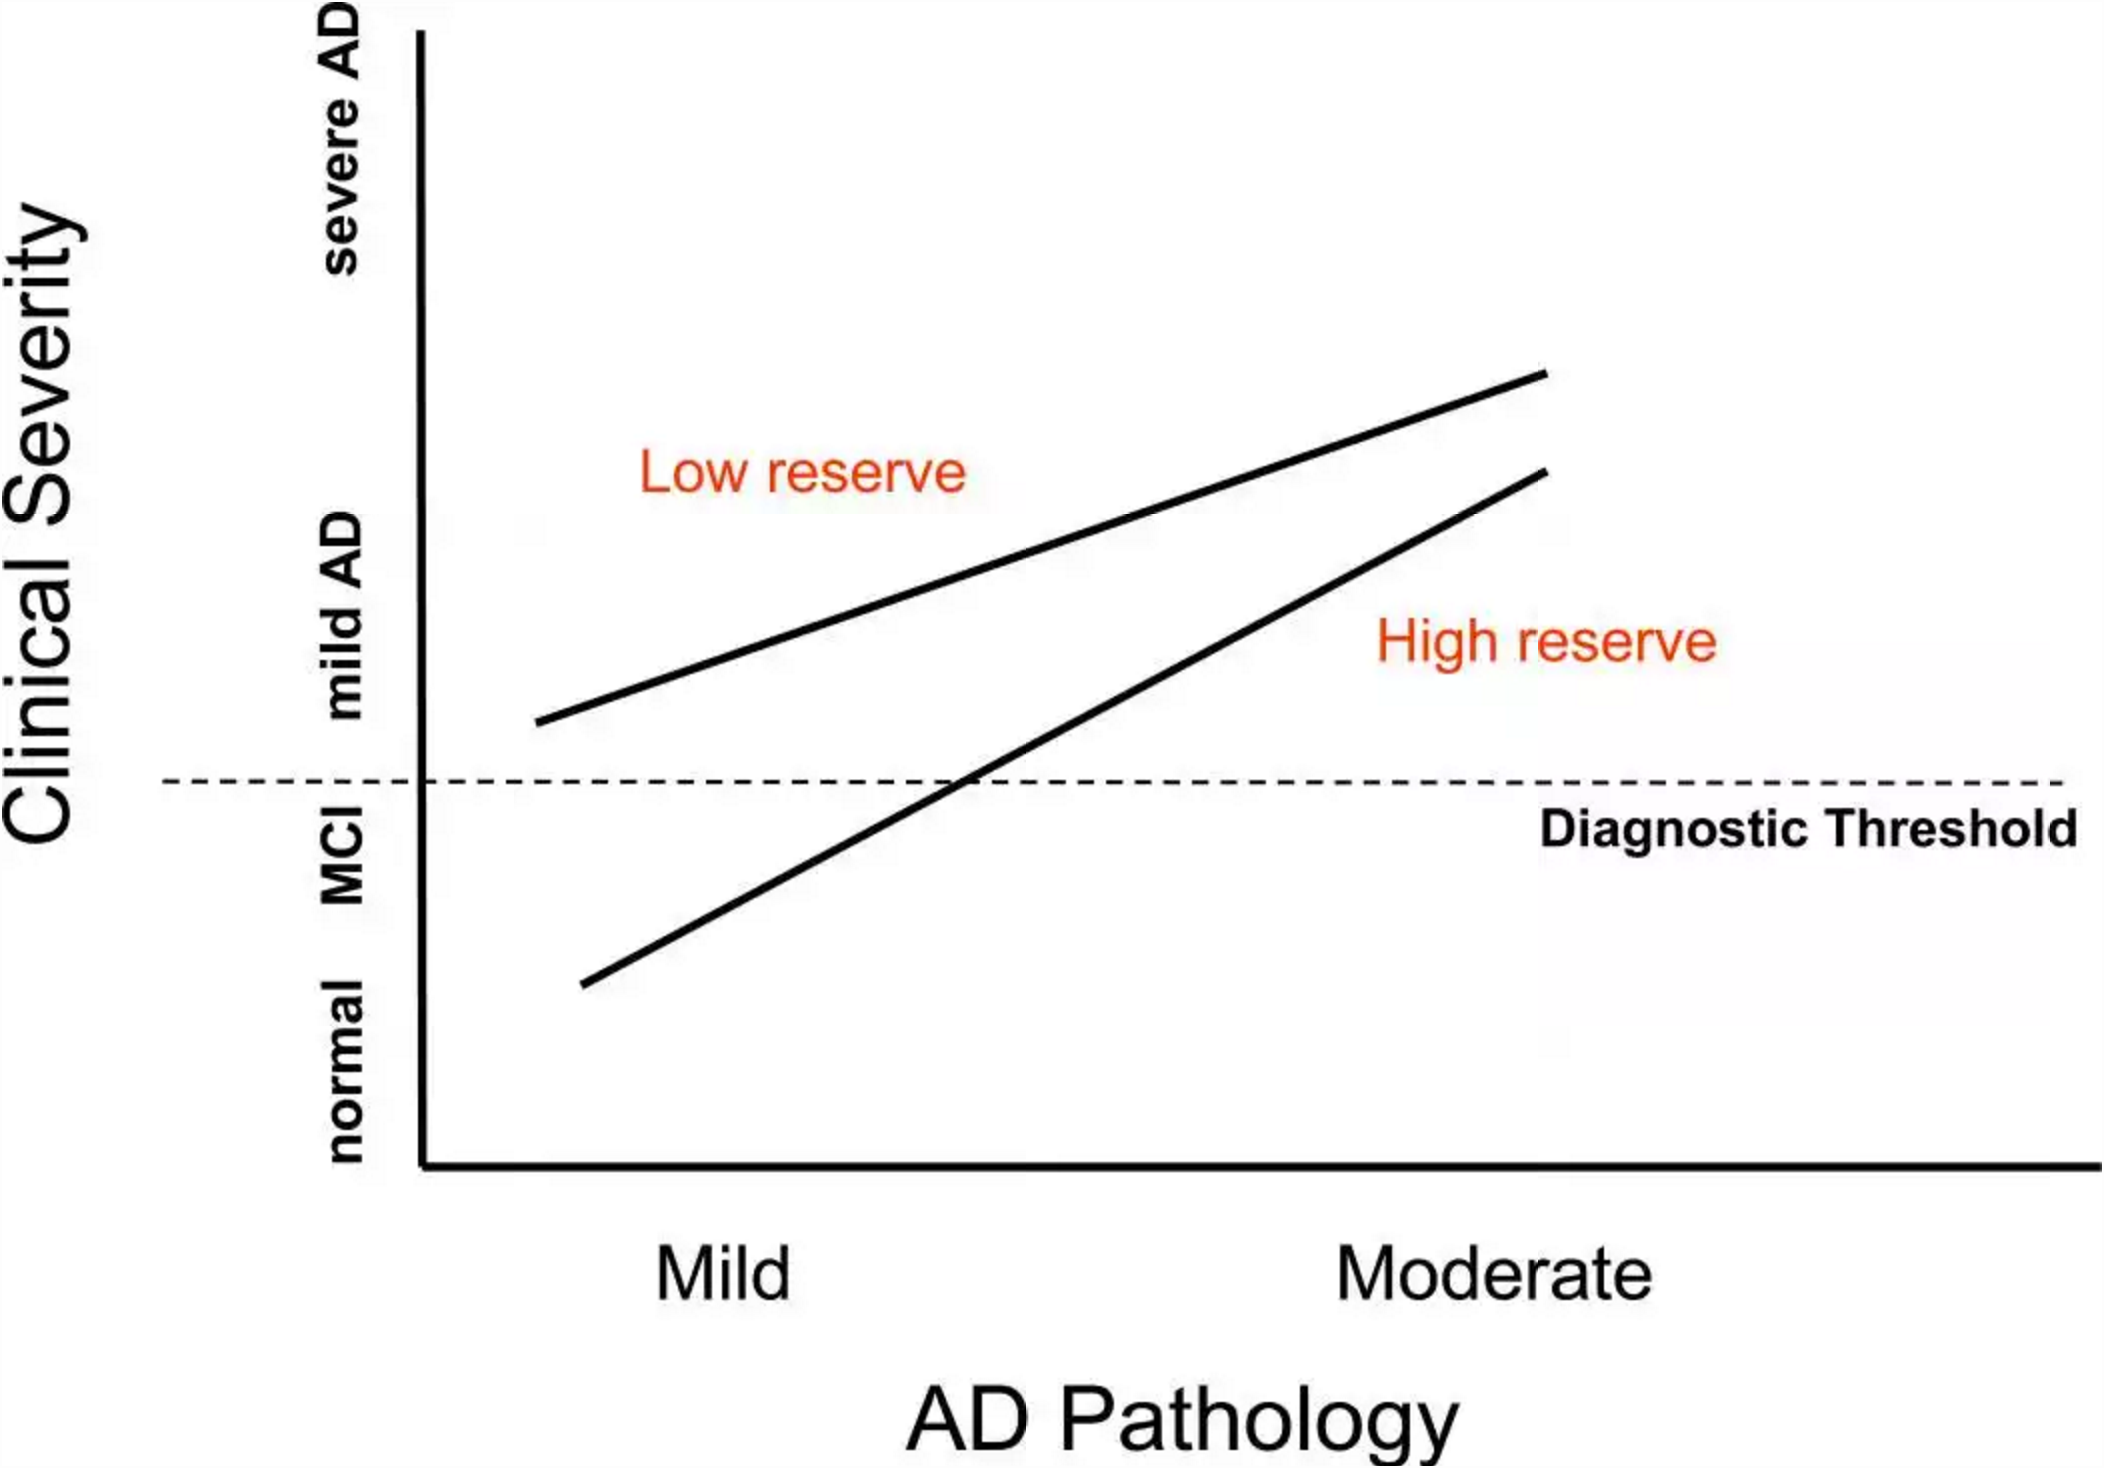
\includegraphics[scale=0.1, angle=0]{Files/literature-review/figures/lancet-neurology-adpathology}
    \caption{Theoretical effects of different levels of AD pathology, on the x-axis, and clinical severity, on the y-axis. Figure adapted from \citeauthor{Stern2012} \citeyear{Stern2012}, previously published in Lancet Neurology journal \cite{Stern2012}.}
    \label{fig: lancet-neurology-adpathology}
\end{figure}


\textbf{Head Injury.}
Those who have experienced moderate to severe head injuries have also been found to have an increased risk of developing AD.

\textbf{Air Quality.}
The quality of air also has an effect on risk. Environmental pollution, or inhalation of smoke can increase levels of free radicals in the body. Free radicals damage all cells, and their danger increases with age. This destructive nature of free radicals is believed to cause cell death in brain cells within AD \cite{AlzheimerEurope2015}.

\subsubsection{Lifestyle Risk Factors}

\textbf{Obesity.}
Having a body mass index (BMI) which is regarded as overweight or above during middle age has been found to significantly increase the risk of dementia onset in later life \cite{Profenno2010}.

\textbf{Diabetes.}
There is a link between diabetes and AD and VD. As such, diabetes brings with it an increased risk of developing dementia. AD patients are typically found to have low insulin levels \cite{Dosunmu2007}. In addition, type 2 diabetes shares the risk factor obesity, and the combination of both has been found to further compound risk \cite{Profenno2010}.

\textbf{Smoking.} As mentioned earlier in environmental risk factors, air quality is drastically reduced when smoking. Smoking is known to increase the risk of many diseases, including dementia through vascular mechanisms.

\textbf{Blood pressure.}
Non-optimal blood pressure (high/low) can also have an effect on the risk of developing dementia \cite{Qiu2005}.

\textbf{Cholesterol.}
Not all cholesterol is created equal. HDL (High-density lipoprotein) is often regarded as ``healthy cholesterol''. Conversely, high levels of LDL cholesterol (low-density lipoprotein) increases the risk of developing both AD and VD.

\textbf{Sleep.}
Poor sleep quality and short sleep duration has been linked to an increase in dementia risk \cite{Tsapanou2015}. This may be due to beta-amyloid levels increasing, a toxic protein which builds the plaques found within AD, due to poor sleep.

\textbf{Stress and Depression.}
Stress and depression are associated with an increased risk of developing dementia\cite{Saczynski2010}. The exact mechanism is not fully understood, however, the physiological and lifestyle changes that occur with stress and depression (changes in blood pressure, sleep quality, diet) may further compound the issue\cite{Schneiderman2005, Tsapanou2015}.

\textbf{Social Interaction.}
Greater levels of social engagement are associated with lower rates of dementia \cite{Saczynski2006, Fratiglioni2000}. Relationship satisfaction is also negatively correlated with dementia risk \cite{Amieva2010}, perhaps due to increased cognitive stimulation and reduced depression \cite{Saczynski2010}.

\textbf{Heavy alcohol use.}
Alcohol has been shown in studies to have a protective effect against dementias, however, large amounts and abuse of alcohol increases the risk of dementia \cite{AlzheimerEurope2015}.

\textbf{Atherosclerosis.}
The accumulation of fats on the artery walls, often referred to as plaques, reduce the blood flow to the brain, often leading to stroke. This reduced blood flow is a cause of VD. AD also has associations with various vascular conditions \cite{Dolan2010}.

\subsubsection{Modifiable Risk Factors}
Many of the identified risk factors associated with dementia can be considered modifiable; meaning that an individual can take conscious action to change their lifestyle, behaviour and environment to mitigate their risk \cite{AlzheimersAssociation2015b}. It is, however, important to recognise that insights regarding modifiable risk factors apply to large population groups, derived from studies that show associations between a factor and a dementia outcome \cite{Baumgart2015}. As such, despite addressing and correcting all modifiable risk factors, some individuals will still acquire dementia, whereas others who do nothing will not. Still, this should not deter the effort to focus on addressing modifiable risk factors across the general population. General understanding of these risk factors by the public, like the condition itself, is low \cite{Farrow2013}. In a study performed by \cite{Farrow2013}, 123 participants were assessed via a survey regarding the aforementioned behaviours and risk factors and its relation to AD risk. The respondents had noticeably less knowledge about the role of physical activity, diet, bodyweight, and diabetes, on AD risk. The study showed that after use of an informative AD website, the participants' knowledge of AD risk factors had significantly improved at the p \textless .001 level \cite{Farrow2013}.

\subsection{Impact on Everyday life}
The impact of the disease is great, not only for the PwD, but also for those closest to them. This also includes their carers, who are often close family members. As mentioned earlier, during the progression in the early and middle stages, the PwD will require additional support for various tasks that they would otherwise be capable of.

\subsubsection{Activities of Daily Living}
ADLs are those which people can normally perform without requiring additional assistance. ADLs include eating, dressing, using the toilet, continence and maintaining personal hygiene (e.g. showering and brushing teeth). During the progression of dementia completion of these ADLs becomes affected, and eventually require assistance. Often before these basic ADLs are affected, a PwD will require additional assistance with the more cognitively demanding Instrumental ADLs (IADLS). IADLS are defined as activities that are not essential for fundamental functioning, however, enable a person to live independently \cite{Bookman2007}. Examples of IADLs include preparing meals, medication management, shopping and money management.
The monitoring of these ADL/IADLs have become an important task to various health care providers \cite{Philipose2004}. By monitoring someone's performance when completing an ADL, it is possible to establish a measure of their health and cognitive well-being. If this measure begins to decline, it is an indication that some intervention may be required and the person's health and care requirements may need to be re-evaluated. Many caregiving and nursing homes record and report their patients' ADLs.
This is typically performed by the caregivers themselves, however, it has been found to be error prone, time consuming and is generally considered invasive by those being monitored \cite{McDonald2001}.

\subsubsection{Medication Management}
Medication management requires many forms of cognitive acuity, such as memory, concentration and future planning. For this reason many people require some form of reminder and scheduling assistance to help them to take their prescribed medication at the right time. The need for a reminder is even more prevalent in those with dementia, who are often prescribed complex drug regimens while also experiencing a decline in their physical and cognitive abilities \cite{Elliott2009}.
Without the use of reminders, adherence rates in the elderly would certainly decline. Adherence to prescribed medication regimens for PwD are important for a number of reasons, not limited to the sub-optimal efficacy of the treatment, however, also financially for the PwD or their family. Studies focusing on adherence rates for chronic conditions found average adherence rates ranging from 43\% - 78\% \cite{Claxton2001, Cramer2003}. Adherence rates for PwD are varied, with those living in full time care having very high rates of adherence, and those living independently having lower rates \cite{Campbell2012a}.  Successful interventions suggest that frequent reminders for PwD can improve adherence, particularly when human communication is used \cite{Campbell2012a}.

\subsubsection{Independent Living}
To live independently, free from the care of others requires autonomy and the ability to act upon decisions safely. Unfortunately, PwD often become a risk to themselves and others due to poor judgement, confusion and forgetfulness. There are many instances in which PwD have reported behaviours which placed them and others at risk \cite{Sandberg2015}, such as causing a fire by leaving a cooking appliance on. As such, assessment of independence is commonplace when caring for someone with dementia \cite{Sandberg2015, GILMOUR2003}. The benefits of residing in a care home are 24/7 access to safe and qualified care and medical staff who ensure ADLs are performed, medications are taken, and provide physical and emotional support. Despite this, 85\% of people would prefer to live at home if diagnosed with dementia \cite{AlzheimersSociety2014}. This desire to remain at home, in familiar surroundings, may be a valid one, considering that 50\% of those admitted to residential care die within 3 years, with almost one third needing palliative care within 1 year \cite{Hjaltadottir2011}. Because of this, many individuals (typically relatives of the PwD) opt to become informal carers, providing regular unpaid care and support.

\subsubsection{Care for PwD}
The role of a carer entails many tasks, and the PwD's wellbeing is their primary objective. Over time, as the condition deteriorates, PwD will become increasingly dependent on their carers, and informal carers often find themselves overwhelmed, ultimately suffering from depression and stress themselves \cite{Mahoney2005}. A day filled with numerous tasks: monitoring the PwD ensuring they do not wander, scheduling and preparing meals, arranging appointments, administering medicines, performing household tasks, and managing emotional and physical outbursts. Whilst a one-to-one care model seems apt for such an involved scenario, a current examination of care standards and staffing ratios showed the worst ratio observed was a 1:64 patient:carer ratio, whilst the best observed was a 1:5 ratio \cite{Harrington2012}. With such a stretched healthcare provisioning model, the standards of care in most countries (except Norway and Sweden) were found to be lower than the levels recommended by experts \cite{Harrington2012}.

\subsection{Technology in Dementia Research}
From analysing the pathology, symptoms, risk factors, management, and quality of care experienced by those with dementia it is apparent that the condition is complex and multifaceted. As such solutions to the issues it causes cannot be found from clinical research alone. Technology-based research within dementia has been a focal research area over the past 10 years. Initially, much effort was spent understanding where available technology could assist the condition, and initial symptomatic treatment solutions were developed, such as basic reminder systems \cite{Hersh1994, Wilson1997, Morris2003}, physical disability assistance \cite{Nugent2008b} and home-based systems aiming to improve independence and safety in the home \cite{Orpwood2005,Nugent2008b}. As time progressed and funding opportunities grew, technology solutions became more elaborate, aiming to tackle multiple issues with a single solution \cite{Zhang2008,Orpwood2005,Cook2007,Nugent2011}. During this period, smart-home technologies, which make use of embedded sensors, were proposed as a suitable and sustainable solutions for monitoring a PwD in their home. These complex solutions, once deployed, initially struggled to handle the complexity of human behaviours, especially those observed in a PwD, who can behave unpredictably. Smart-home solutions have since improved somewhat through further research, and their use in dementia care is still an active research area \cite{Amiribesheli2015,Wilson2015a}. Much of the research performed on technology in dementia has been focused on the treatment of the condition; relieving symptoms, easing burden, increasing safety and improving care provisioning \cite{xhafa2015, Gillespie2012, Cahill2008}. Recently, it has become apparent that there may be an opportunity for technology in the prevention effort against the condition. \citeauthor{Mangialasche2012} noted that a promising strategy for preventing dementia would be to implement an intervention program that takes into consideration the multifactorial nature of dementia \cite{Mangialasche2012}. Technology may therefore the key to deliver such an intervention to the masses through its ubiquitous reach.

\section{Treatment: Current State-of-the-Art} \label{section: treatment-stateoftheart}
As previously discussed, the use of technology in the dementia epidemic may be categorised into the areas of treatment and prevention. Treatment refers to the use of the technology to alleviate issues caused by dementia, and also symptomatic aid, rather than a curative effect.
This Section will discuss the state of the art in this area, highlighting the benefits, current limitations, and the opportunities for improvement.

\subsection{Smart-homes}
Smart-homes and their supporting software systems are the cutting edge of treatment solutions for dementia. Previously only accessible to those in the research domain, smart-home technologies are slowly being refined and developed for the consumer market. These include automated products that can increase home security, control heating, lighting, and detect spoiling food in a smart fridge \cite{Hoy2015, IControlStateofArt2015}. Many of these consumer grade products do not meet the additional demands that a PwD creates. As such, smart-home systems that specifically address these specific needs are very much still within the research domain. Much focus has been placed on the monitoring and assistance of ADLs, using a variety of sensors and machine learning algorithms \cite{Cook2007, Cook2012, Hoey2007, Hoey2010, Chen2012}. The detection of harmful incidents, such as unexpected falls in the elderly, is also a prominent research area in the field of smart-home applications \cite{Chaquet2013,Yang2010}. Other uses include the detection and subsequent redirection of pacing, a common occurrence in which PwD become restless and walks in an attempt to perform various purposeless activities \cite{Nugent2011}.

\subsubsection{Complexity}
Despite the numerous potential uses many of these solutions fall victim to the sheer complexity of human behaviour, along with interoperability and scalability issues \cite{Cook2007, Tang2010, Lim2008}. Along with this, a unified vision and understanding of who `smart-home' users are, and how they might use the technology is missing from ``a field being overwhelmingly pushed by technology developers'' \cite{Wilson2015a}. In addition, many of the algorithms and proposed solutions, despite providing promising accuracies in technical tests, have not been efficiently trialled in valid scenarios with PwD, and as such their true efficacy has not been assessed \cite{Dawson2015, Lyons2015}.

\textbf{Benefits.}
Reduce caregiver burden; Increased PwD safety; Assistance with ADLs; Remain at home longer.

\textbf{Limitations.}
System complexity; Cost of installation and maintenance; Scalability issues; Not Readily Available; No evidence-based RCTs.

\subsection{Cognitive Aids}
Failing memory and ability to plan is undoubtably a prominent feature of dementia. As such, there is an opportunity to improve memory and planning using cognitive aids, such as reminders and scheduling tools. Reminder systems for the cognitively impaired have evolved with the technology, and now range from the simpler time-specific reminders to complex context-aware reminder systems, incorporating numerous environmental sensors \cite{Hersh1994, Zhang2008, Zhou2012}. Reminder systems to aid scheduling can be classified into 4 main groups, based on the type of information used to issue the reminder: (1) time-based, (2) location-based, (3) activity-based and (4) hybrid reminder systems \cite{Seelye2012, Hartin2014-IWAAL}.

\subsubsection{Time-based}
For PwD time-based scheduling is the most rudimentary and the most commonly implemented. NeuroPage \cite{Hersh1994, Wilson1997} is one such example. It was designed to be used by persons with memory impairments as a result of brain injury, however, could also be used by those with progressive conditions, such as dementia. Time-based reminders whilst extremely reliable face the issue of delivering reminders during inconvenient situations, such as when the user is eating, working or in a different location from the reminding device. These types of situations can cause a person to experience stress and increased frustration, given that they feel obliged to address the alerts \cite{Mark2008}, which can only be exacerbated with dementia symptoms.
Consequently, location and activity based reminders aim to observe and avoid these types of situations, opting for a model which prioritises the current observed activity or location for the delivery of a reminder, rather than the time.

\subsubsection{Location-based}
Location-based reminders use an individuals observed location to influence the delivery of a reminder. The use of location information has taken many forms both inside the home, and outside. \citeauthor{Marmasse2000} pioneered the use of GPS to deliver location-based messages to a mobile device when the device was in proximity to a pre-programmed target, e.g., a shopping list sent when near a store \cite{Marmasse2000}.
Whilst building upon simple time-based solutions, the limitations of these systems are that they are typically restricted to one format of prompt (e.g., text or voice instructions), do not consider other available contexts (e.g., activities, time) and as such are incapable of avoiding delivery during inappropriate times, or during complex activities (e.g., driving at night) \cite{Seelye2012}. \citeauthor{Tu2013} addressed some of these issues in their iReminder solution, which was capable of predicting a user’s future location based on previous routes and delivered a location specific reminder before they arrived, thus potentially minimising inappropriately timed messages \cite{Tu2013}. These models and techniques, whilst originally based outside the home, have been applied to the technology and dementia paradigm. The introduction of GPS in dementia care took the form of geofencing \cite{Wang2015}, enabling carers to be alerted when a PwD left a pre-set boundary, such as wandering from their home in the middle of the night. Inside the home, however, it is very difficult to track the PwD's movements, due to minimal, or nonexistent GPS signal. As such other methods have been developed to track the current location of people within the home, including pressure sensors, infrared and Wi-Fi signal strength \cite{Chen2012}. Again, reminder solutions for PwD in the home, using location as their primary context also experience the same limitations, with the additional complexity of PwD behaviour \cite{Grunerbl2011,Lin2014a}.

\subsubsection{Activity-based}
Activity-based reminders offer a potential solution to the complexity of a PwD's unpredictable daily schedule. Rather than prescribe a one-size-fits all time-based reminder system, activity-based systems aim to learn or deliver pre-programmed reminders when certain activities are detected. For example, these proposed systems could remind a PwD to turn off the oven or take specific medications once a meal has been prepared, increasing safety and medication compliance.
Activity-based reminders rely heavily on the field of pervasive computing and activity recognition, a field which aims to detect people's activities and behaviours. Home-based activity recognition typically makes use of an array of sensor modalities, which include contact, pressure and heat sensors, infrared movement detectors and varying formats of video \cite{Chen2012b}. Accounting for these varying types of data increases the complexity of the system, however, when performed correctly, can also increase the accuracy of the activity classification. Within the dementia care paradigm, activity recognition is proposed to monitor ADLs, assess their progression and provide assistance or prompts (reminders) when needed. Systems that use one sensor modality are much more scalable, however, are somewhat limited to the classification of actions, e.g., opening a cupboard door, rather than the overarching activity \cite{Chen2012b, Patterson2015}. If a system is to understand why the cupboard door has been opened, then additional input is required to increase the systems understanding \cite{Chen2012}. As such, the current approach to activity-based reminders require a number of sensor modalities and accompanying machine learning models to infer activities accurately. Autominder \cite{Pollack2003} is an activity-based reminder system that uses artificial intelligence techniques and quantitative temporal Bayesian networks to observe and reason about ADLs using a robot, which have been performed to develop a model of an elder’s typical daily plan. The system maintains and uses this model to schedule future reminders, however, once a given schedule is learned, it cannot be altered.
The limitations of these approaches are shared with the smart-homes described earlier, in that they are expensive to purchase, install and maintain, suffer scalability issues \cite{Wilson2015a} and any sensor failure greatly impacts the systems visibility and thus reliability \cite{Ye2015}.

\subsubsection{Hybrid}
Recognising the insight that each context brings, hybrid solutions aim to utilise all available contexts, optimising accuracy by selecting the most appropriate for any given situation. Such a goal is admirable, however, highly complex. Many frameworks and architectures have been proposed, however, suffer from the same issues; scalability, complexity and variability. Whilst rules may be used to discern which contextual input is more appropriate in each scenario, the list of scenarios can be infinite, and even so, these rules will vary from one PwD to the next. The COGKNOW project  proposed a complex context-aware system for persons with mild dementia \cite{Zhang2008}. The architecture incorporated time, location and user activity as contexts, along with the time that the to-be-prompted activity was typically performed. The full feature set of the system was, however, not realised upon the project’s close. iConAwa, proposed by \citeauthor{Ylmaz2012}, was another intelligent context-aware system proposal which aimed to provide smartphone users with context-aware information and services \cite{Ylmaz2012}. The paper presented a set of novel case studies, in which a number of users with a number of interests received prompts related to services which may be of interest. The system used location, time, network connectivity and user preferences as contexts.  The entire system was based upon a complex, user maintained, rule-based ontology, encoded in OWL (Web Ontology Language). Despite a novel and promising framework, the solution was never developed, deployed or evaluated.

\subsection{Reducing Complexity}
Much of the research in this area has been driven by the technology sector, forsaking patient needs for technical complexity.
The need for a PwD is to be given the appropriate reminder, at the appropriate time, in a manner they can comprehend. This need has become obscured over time, and has slipped into an approach of constructing the most elaborate systems, with each iteration becoming more complex and technologically novel, albeit lacking any real merit for the end-user. None of the aforementioned studies or systems considered how delivery of the reminder may interrupt the user, nor did they alter the delivery based on existing evidence, extracted from past acknowledgment rates \cite{Hartin2014-WAGER}.

\subsection{Areas for Contribution}
There is therefore the opportunity to reduce complexity and increase efficacy in reminders for PwD. Chapter \ref{chapter: treatment-framework} addresses these areas using a simpler approach; a smartphone app to monitor acknowledgement rates to temporal-based reminders, learning usage patterns through the embedded sensors, with the aim of improving reminder delivery and adherence for each individual. Chapter \ref{chapter: treatment-framework} details the development of the reminding solution and preliminary testing with a healthy cohort. Chapter \ref{chapter: treatment-framework} details the results from usage of the app by over 30 PwD in a 12 month trial. Sensor based reminding is also then optimised for this particular cohort and future improvements are discussed.

\section{Prevention: Current State-of-the-Art}
To date, technology's opportunities in the dementia epidemic has almost exclusively been in the area of treatment. Recently, prevention of the condition has been identified as a priority. With the advent of wearable technologies and increasing smartphone usage and capabilities, a new opportunity has arisen to use these tools to focus on the prevention of the disease.
This Section will discuss the shift of focus to prevention, the current state of public health campaigns and technology's role, and also the state of the art in smartphone and wearables.

\subsection{Adjusting the focus to prevention}
During the course of study into dementias, and attempts to develop a cure, various risk factors have been discovered and extensively studied \cite{Baumgart2015}. This work resulted in sentiments which claimed that whilst dementia was not curable, the clinical evidence suggested that it was preventable in many cases \cite{DelaTorre2010,Willis2013}. The AD research community responded by addressing government bodies at the G8 summit in 2013, requesting that AD prevention be placed as a major health aim, and calling for others to further study the risk factors associated with the condition \cite{Smith2014}. Advances since have suggested that the management of modifiable risk factors may hold the key to dementia prevention, especially for AD and VD \cite{Solomon2014, Lovden2013}. Many of the risk factors identified can be addressed by simply improving ones general health;improving diet, increasing exercise, improving sleep quality and reducing stress. Since the development of public health in classical Greece, improving the general health of the population has been a key objective \cite{Ozonoff1994}. In the modern era, many public health campaigns have aimed to improve the general health of the population to mitigate future risk and treatment costs of specific diseases, such as heart disease, stroke, diabetes and obesity \cite{Labarthe2014, CentersforDiseaseControlandPrevention2015}.

 \subsection{Public Health Campaigns}
Whilst the need for a public health campaign for dementia risk is obvious \cite{cook2014public}, the most effective delivery method is not. In recent years, ICT has been increasingly used to extend the delivery of public health campaigns \cite{Mirarchi2015}, and in some cases, used as the primary method of delivery \cite{Hattink2015}. These ICT enabled campaigns typically utilise the world wide web as their platform for distribution. Often they may take the form of a static webpage which displays information about a condition, current prevalence, generalised risk statistics, and various steps to improve outcomes \cite{AlzheimersAssociation2015a}. This model is effective for a number of reasons, with accessibility being the primary advantage over classical approaches. Information is generalised and presented in a clear and concise manner, it is accessible at any time, and on a variety of internet ready devices, however, it is up to the user to understand the information and enact upon any recommendations provided, which is where the efficacy of this approach begins to experience its limitations. Whilst the information is accessible, it is generalised and non-specific to the reader which can lead to confusion and non-adoption of the recommendations \cite{lerouge2014challenges, Tones1994}. It has also been found that may of these websites suffer from poor readability \cite{RisoldiCochrane2012}, which may result in sub-optimal learning outcomes. The authors of this research suggest that additional effort be made to ensure that all health information communicated is easy to read and understand \cite{RisoldiCochrane2012}.

\subsubsection{Increasing Interactivity}
One possible approach to improve the understanding and subsequent adoption of any public health recommendation is to improve the interactivity of the content. Increasing interactivity online has been shown to improve learning outcomes, especially if the content is perceived as being useful \cite{Oh2015, Wei2015}. Evolving from the static webpage model described earlier, an education portal provides a structured learning approach, using teaching modules to guide progression through content, and often utilise interactive tools such as glossaries, pop-quizzes and games, to help boost understanding \cite{Hattink2015}. This portal approach has been successfully applied in the past to educate informal carers of PwD, from various levels of education, about the condition and provide advanced caregiving and coping techniques \cite{Hattink2015}.
Whilst often more interactive than static information pages, the education portal solution can add unwanted complexity for the user, requiring an active internet connection to use and typically requiring account registration to use the platform.
Smartphone apps provide an opportune platform to deliver educational information with an interactive component. Touch interfaces have been found to be more engaging for learning purposes \cite{Jones2006}, and due to user-design guidelines provided by Apple and Google \cite{AppleNotifications2015,GoogleAndroid2015}, the quality of interactive apps is ever increasing. It has become the status-quo to provide highly interactive features in the most basic of apps. Nevertheless, the availability of apps or mobile ready content has been found to be considerably low within public health. One study of 55 American health websites found that only 22\% (n=12) were considered mobile ready, of which only one-third had better or similar readability to their traditional website counterparts \cite{Cunningham2015}.

\subsubsection{Health Campaign Apps}
With 2015 being the year in which smartphones surpassed personal computers as the most popular method to access the web, it is suggested that public health campaigns recognise this shift and adapt accordingly \cite{Cunningham2015}. Anticipating this shift, the US Centers for Disease Control and Prevention (CDC) were one of the biggest public health authorities to 'go mobile' in 2013, by launching a free public health app service on the Google Play store and Apple App store \cite{CentersforDiseaseControlandPrevention2013}. This prompted a surge in the development of public health apps, published from various leading authorities including the United Nations \cite{UnitedNations2015}. These public health apps include helpful tools to schedule vaccines \cite{CentersforDiseaseControlandPrevention2015b}, apps which encourage swimming as a form of exercise \cite{CentersforDiseaseControlandPrevention2015a}, information on diet when travelling to avoid travellers’ diarrhoea \cite{CentersforDiseaseControlandPrevention2015c}, and even an app which advises on the correct angle of a ladder to minimise the risk of falling injuries \cite{NationalInstituteforOccupationalSafetyandHealthDivisionofSafetyResearch2014}. Whilst these apps are from credible sources and contain valid information, they are not end-to-end solutions designed to measure any change at an individual level, such as the adoption of suggested behaviours or monitoring health metrics.
The technology to perform these tasks does exist and comes in a variety of forms. There is therefore, an opportunity to advance these public health campaigns, and enable them to engage with the population more effectively at an individual level.

\subsection{Everyday mHealth}
The use of technology to monitor everyday health is a thriving area, both for researchers and consumers alike. Currently, there are over 165,000 health and fitness smartphone apps available, and over 280 wearable devices aiming to seamlessly monitor health \cite{IMSmHealth2015}. Many of these apps and devices can be used for the purposes of mHealth (Mobile Health), an area which advocates the use of mobile (including wearable) devices to support the practice of medicine and public health \cite{Adibi2015}.

\subsubsection{Smartphones and app}
mHealth apps are quickly becoming the go-to tools for condition monitoring, providing a convenient and cost effective way for individuals to measure many vital signs, including pulse rate \cite{Led2015, Baig2013}, blood-pressure \cite{Moser2015}, blood-oxygen \cite{Led2015, Moser2015} and also blood glucose \cite{Moser2015}. In addition to these cardiovascular measurements, the smartphones camera may also be used to perform eye \cite{Maamari2014}, ear \cite{Rappaport2015}, and dermatological examinations \cite{Kassianos2015}. Physicians are increasingly using these validated applications in their practices \cite{Topol2012}, however, not all mHealth apps are created equal. The number of health and wellness apps available has more than doubled since 2013, yet many have no scientific evidence base. Figure \ref{fig: imshealth-mhealthapps} shows the type distribution of mHealth apps currently available  in the app marketplace.

\begin{figure}[h]
    \centering
    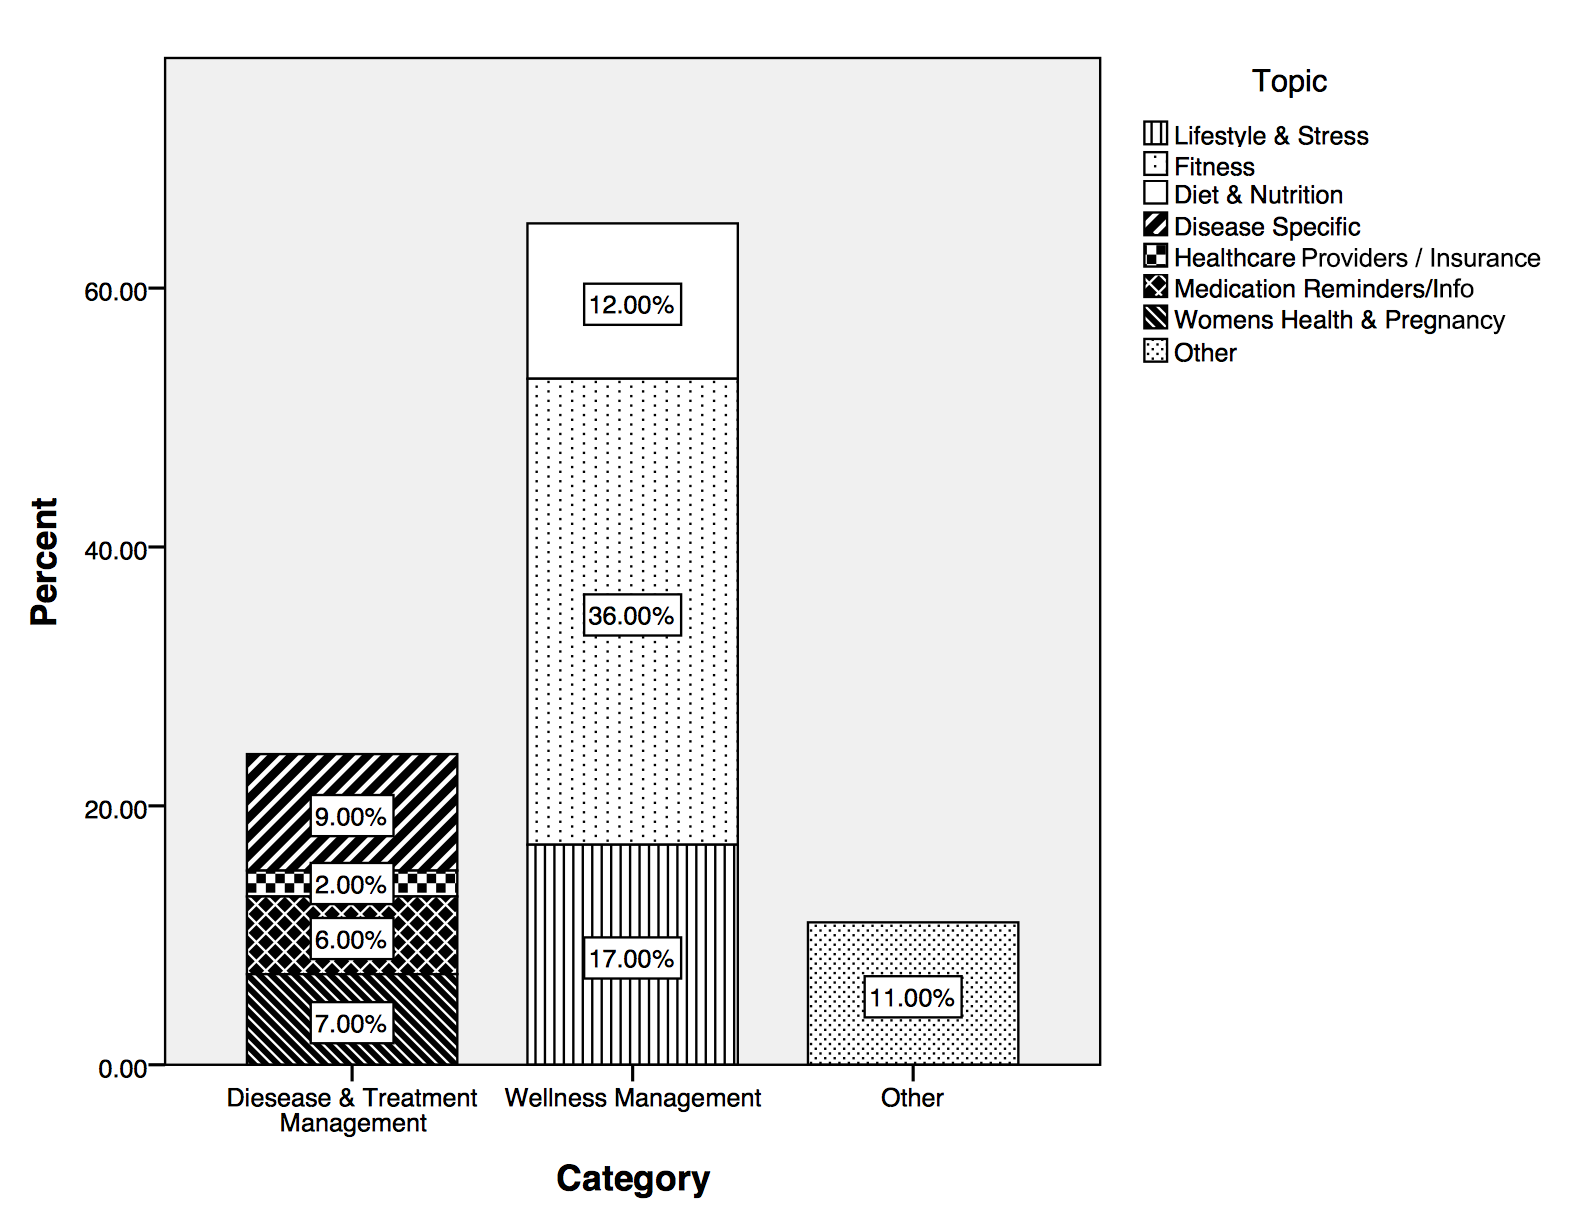
\includegraphics[scale=0.25, angle=0]{Files/literature-review/figures/imshealth-mhealthapps}
    \caption{Categories of mHealth apps available on iOS and android app stores in 2015; data adapted from \cite{IMSmHealth2015}.}
    \label{fig: imshealth-mhealthapps}
\end{figure}

The majority of these apps are categorised as ``wellness management'' apps, of which fitness apps, contribute the greatest to the overall number. Recent articles published in the British Medical Journal (BMJ) \cite{Husain2015} and the Journal of the American Medical Association (JAMA) \cite{Kuehn2015} raised concerns due to the lack of process when publishing a healthcare app on app marketplaces. As a result the vast majority of ``health apps'' have not been assessed by any credible bodies for the information or methodologies that they disseminate. This fact alone stands to cripple the widespread adoption of mHealth solutions due to providers, and consumers, views regarding lack of evidence and credibility \cite{IMSmHealth2015}. There is therefore an opportunity for technology researchers to develop healthcare apps, whose methods are underpinned by clinical literature and evaluated scientifically, to demonstrate the potential impact of widespread adoption.

\subsection{Wearables}
Wearable devices have seen considerable adoption in recent years, driven by demand in the fitness market. The majority of these devices (\textgreater50\%) have been designed to be worn on the wrist, around a quarter are designed to be worn around the chest, and approximately a fifth are designed to worn in the pocket, shoe or purse, as shown in Figure \ref{fig: imshealth-wearableposition} \cite{IMSmHealth2015}. Wearables, despite being standalone devices, often require a smartphone app to sync, extract, and analyse collected information.

\begin{figure}[h]
    \centering
    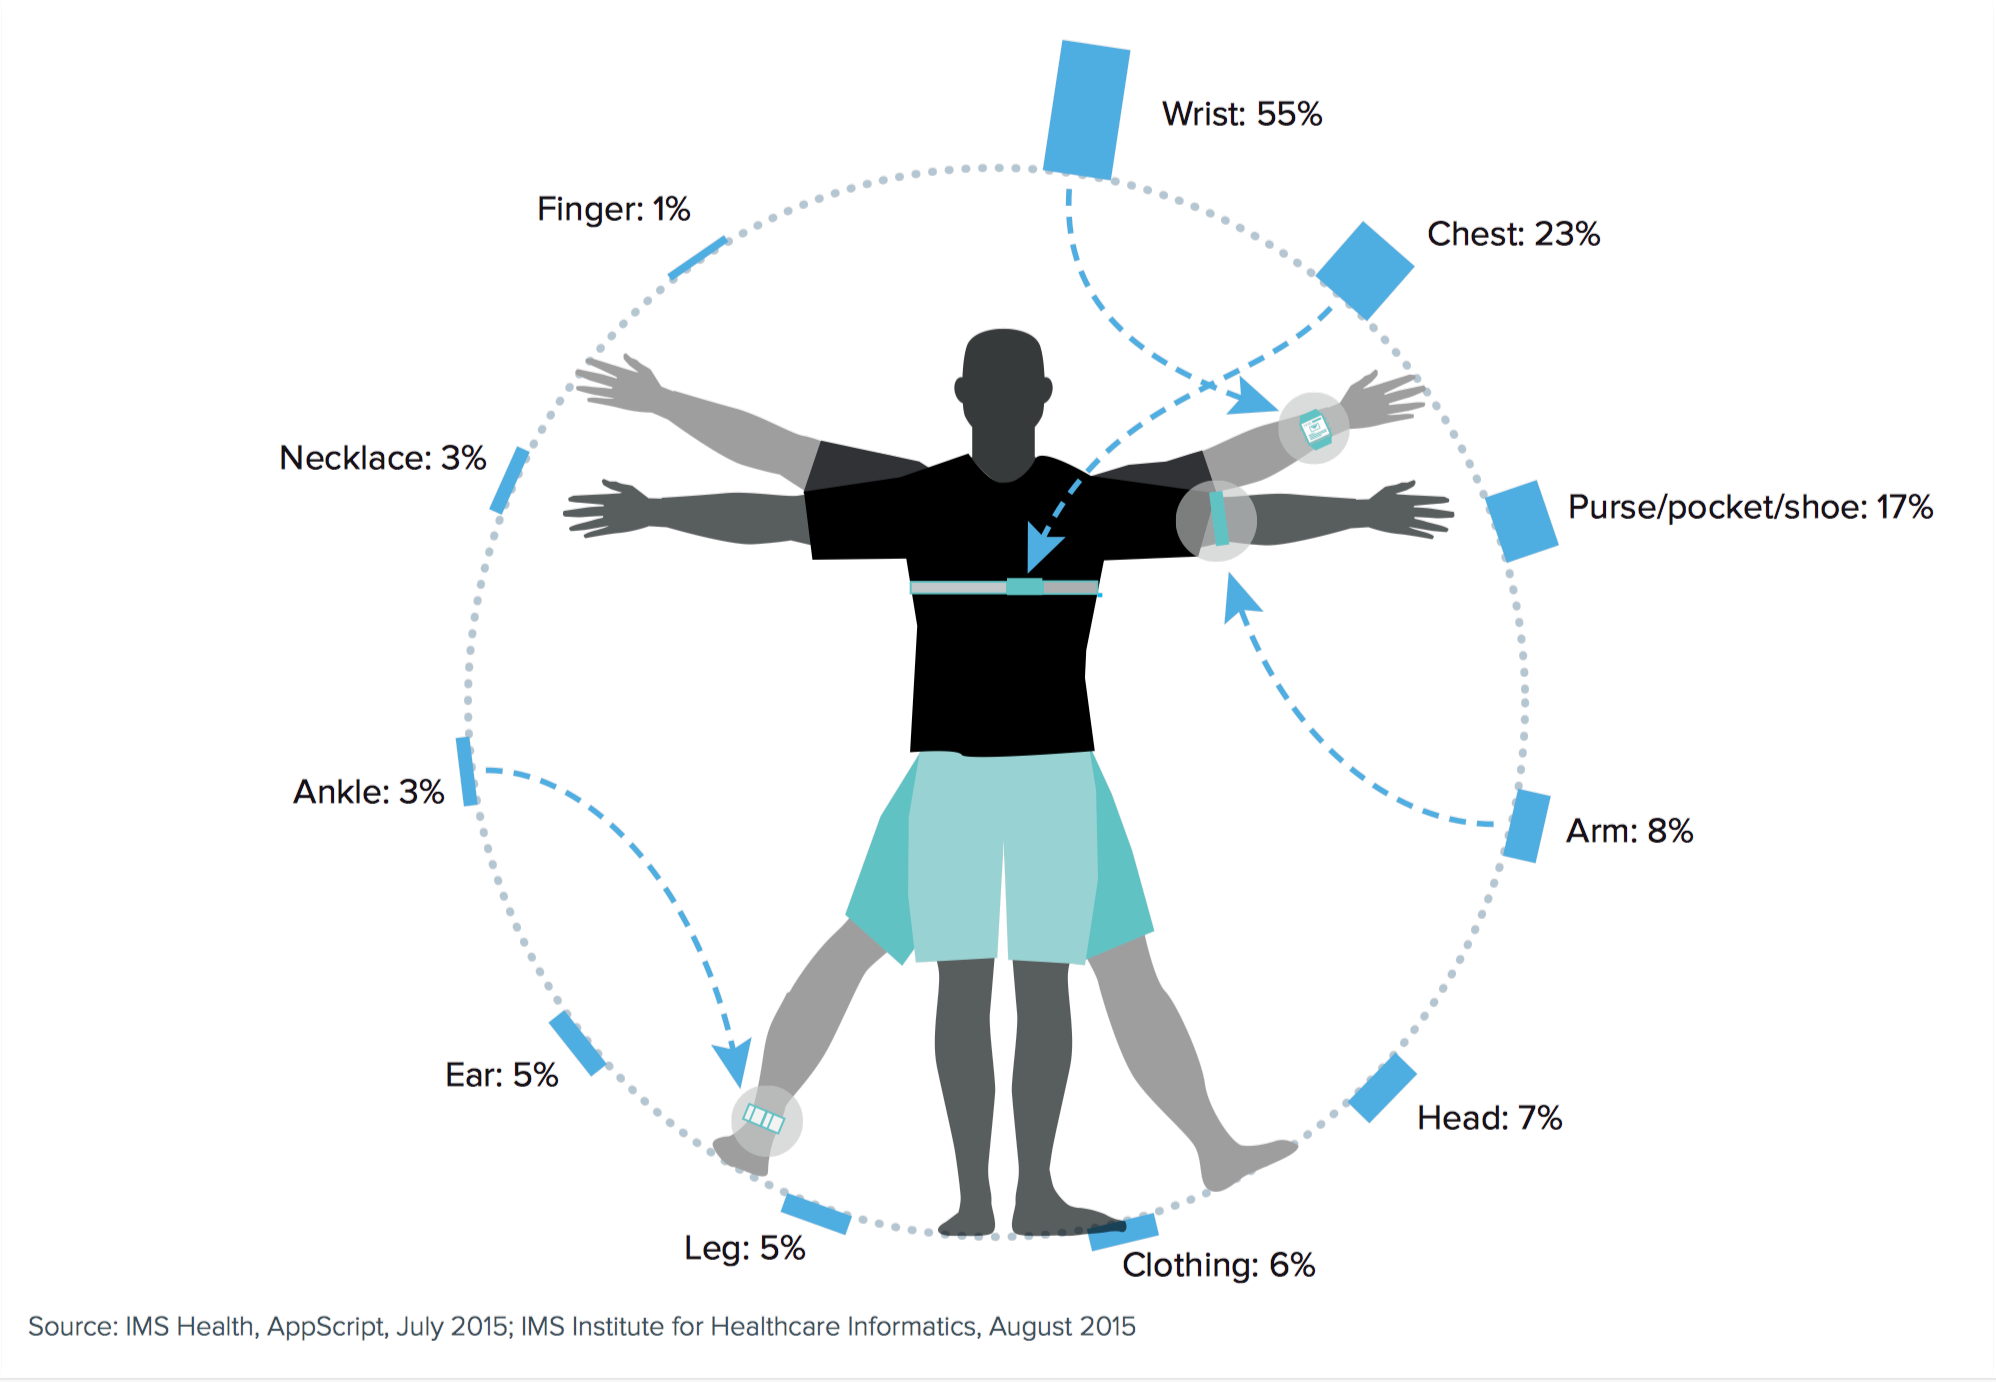
\includegraphics[scale=0.2, angle=0]{Files/literature-review/figures/imshealth-wearableposition}
    \caption{Placement of portable and wearable devices as found by \citeauthor{IMSmHealth2015}. \textit{Source: IMS Health, AppScript, July 2015; IMS Institute For Healthcare Informatics, August 2015} \cite{IMSmHealth2015}.}
    \label{fig: imshealth-wearableposition}
\end{figure}

Similar to the type distribution of mHealth apps, wearable devices targeting general fitness accounted for the largest number of wearable devices in an analysis study by \cite{IMSmHealth2015}. This is presented in Figure \ref{fig: imshealth-devices}. Unlike mHealth apps, however, there are greater barriers to market entry, notably the mass production of hardware, marketing, and research and development. As a result, the standards of available solutions are high, with many device's accuracy claims being independently evaluated and validated by academics \cite{Ferguson2015}.

\begin{figure}[h]
    \centering
    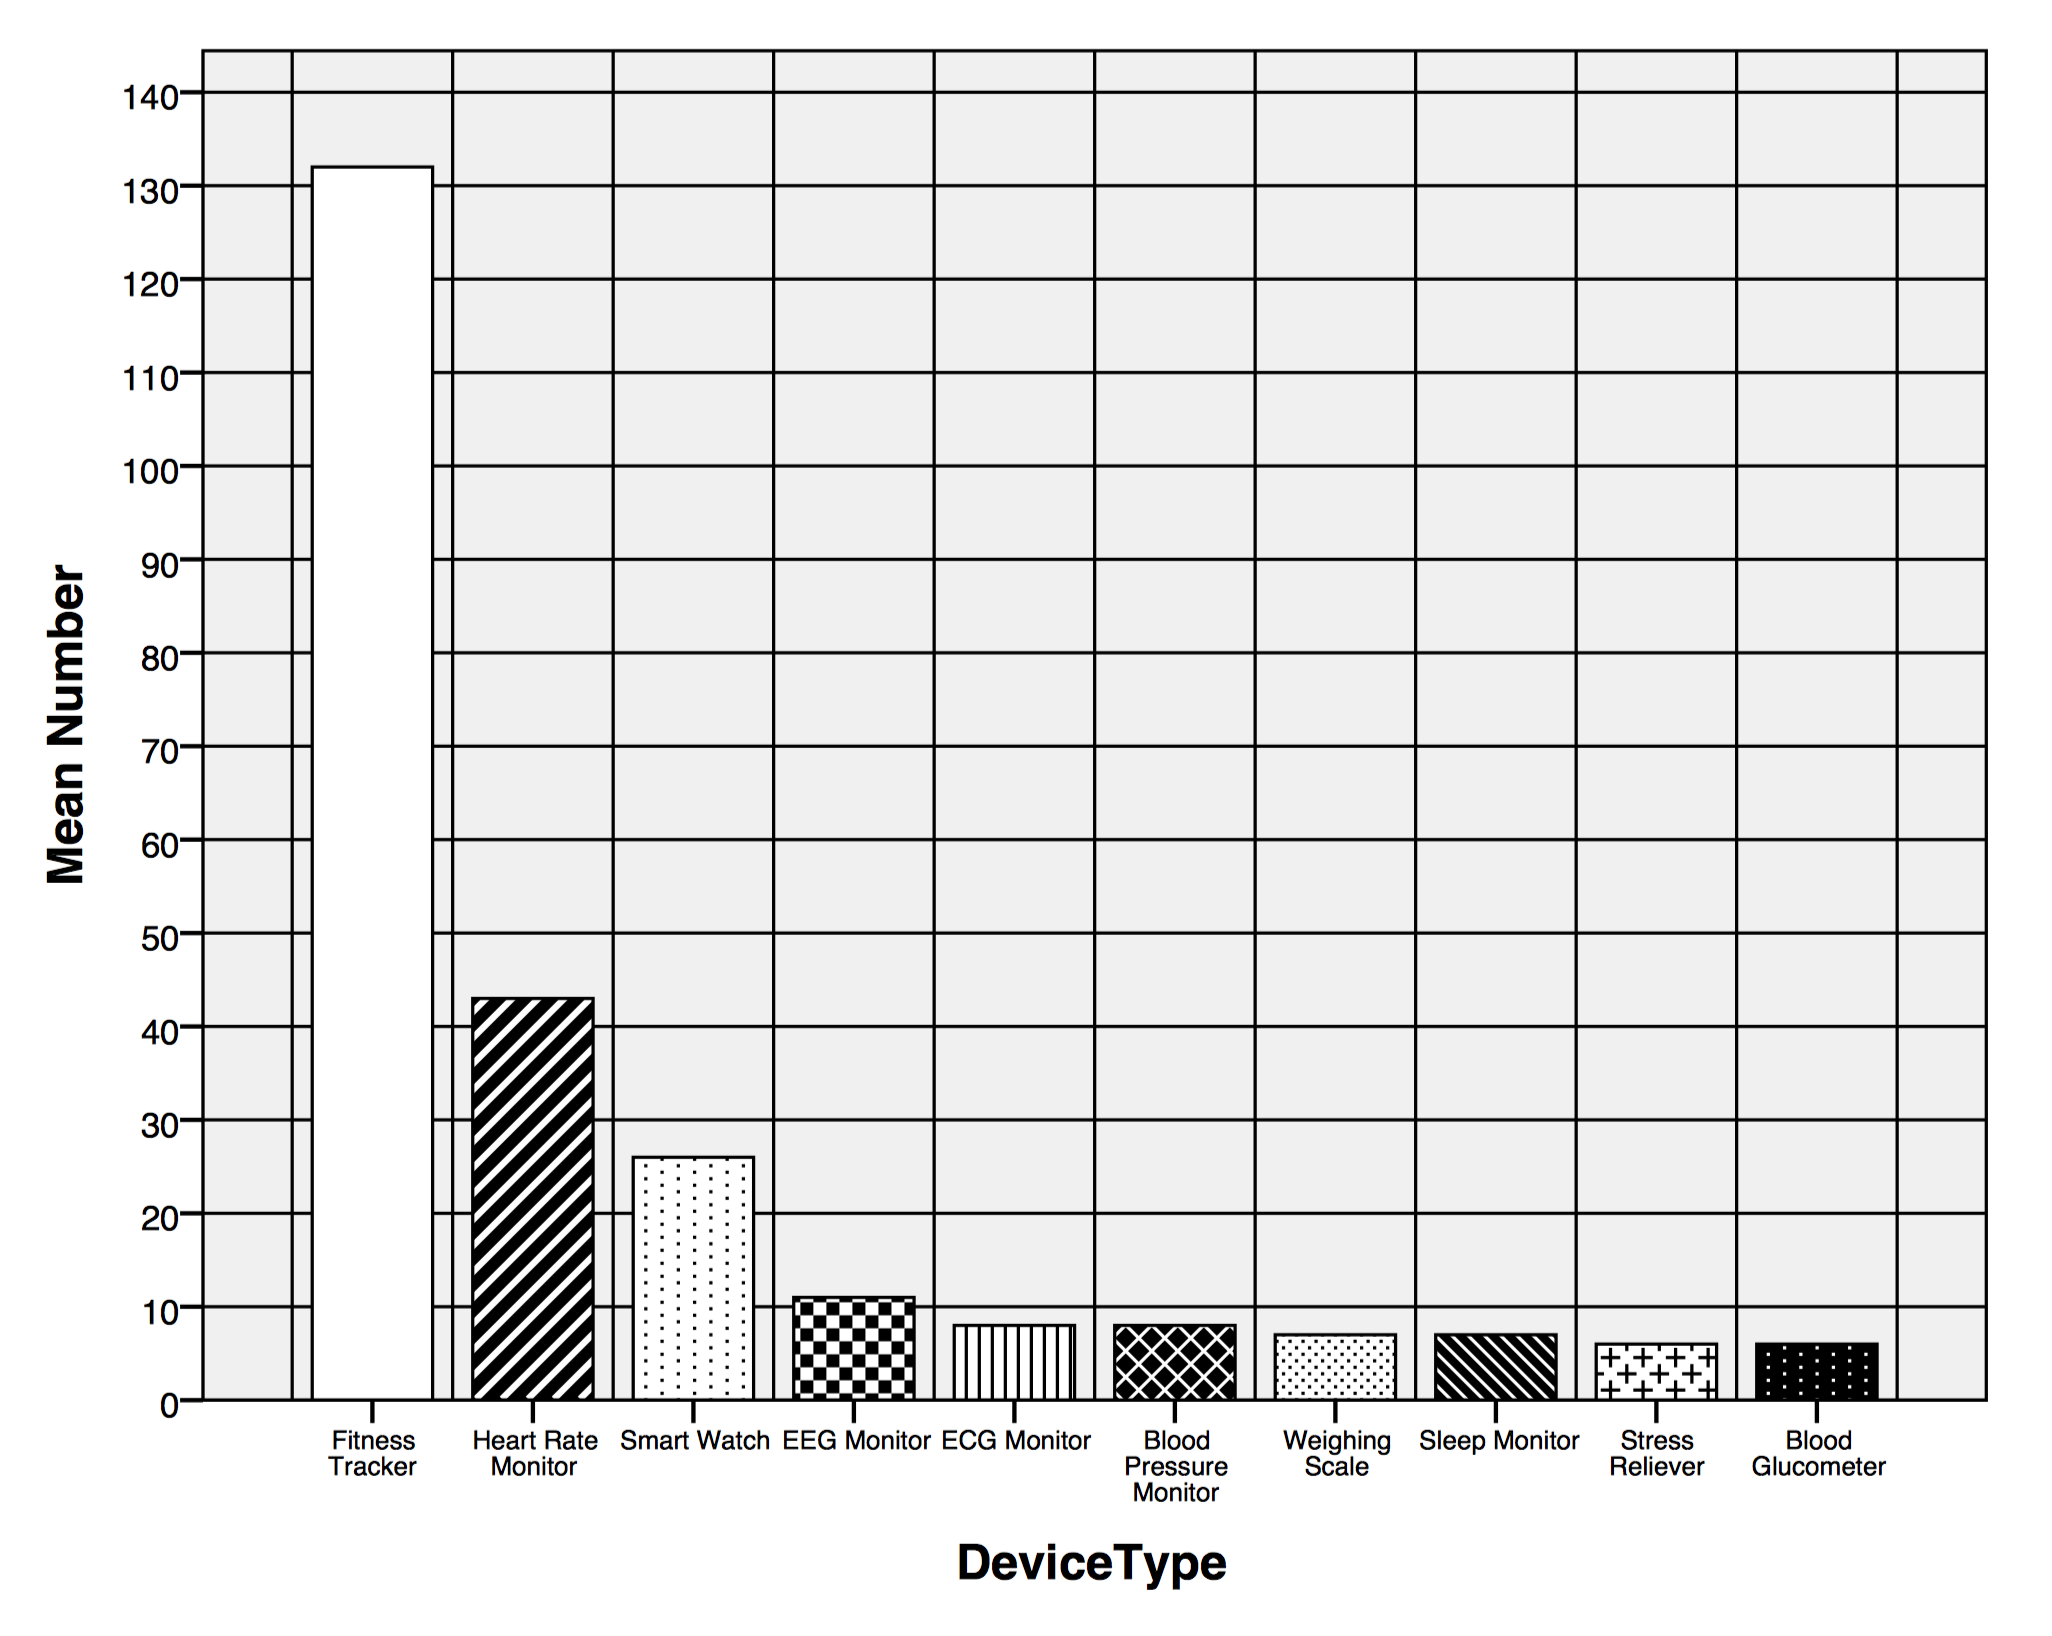
\includegraphics[scale=0.35, angle=0]{Files/literature-review/figures/imshealth-devices}
    \caption{Availability and type of dedicated health and fitness devices; graph adapted from data in \cite{IMSmHealth2015}.}
    \label{fig: imshealth-devices}
\end{figure}

\subsection{Health Monitoring Functions}
Many functions provided by wearable devices and smartphone apps are shared, due to shared hardware, yet each platform can be more suitable than the other in specific scenarios. For the purpose of overall health monitoring, the functions of physical activity monitoring, vital signs monitoring, diet management, sleep assessment and coaching are investigated further.

\subsubsection{Physical Activity}
Physical activity can be monitored by smartphones and wearables in a variety of ways, including the use of embedded sensors. The most commonly implemented feature across all devices is the step counter.

\textbf{Step-Counter.}
Accelerometers and gyroscopes embedded in smartphones and wearables can be used to detect stepping patterns, enabling the devices to be used as pedometers. Originally implemented by independent developers, step-counters have become a standard feature of smartphone devices, with native functions built into the operating systems of both iOS and Android \cite{Orr2015}. Step-count can be a useful measure of overall physical activity performed in a set period (i.e. number of steps per day). As such, it is used as a primary measure in most wearable devices, with daily step count goals established via software. Many evaluations of accuracy have been performed for smartphone and wearable pedometers \cite{Cleland2012, Cleland2013, Yang2010}, including comparative studies \cite{El-Amrawy2015}. Despite similar accuracies, it is often the case in real-world scenarios that smartphones are not present on a person 24/7, and as a result will miss a number of instances.

\textbf{GPS.}
Using GPS it is possible to increase the accuracy and granularity of physical activity data. Especially useful for monitoring distance sports such as running and cycling, it is possible to track the location history of an individual, distance travelled, establish speed, and estimate calorie expenditure \cite{Zhan2012, BUTTE2012}. This gives a much deeper insight into the physical activity performance, however, but for the purpose of general physical activity GPS is superfluous and will cause excessive battery drain in both smartphones and wearables \cite{BUTTE2012}. In addition, loss of a GPS signal when travelling indoors will result in missing or inaccurate data. Due to this, it is recommended that GPS only be enabled for distance and speed specific activities.

\textbf{Self-reporting.}
There are a number of scenarios where it would be inappropriate to use wearables or a smartphone to track physical activity, e.g. swimming and contact sports. In these cases many solutions allow for self-reporting of activity. Using existing and validated data, it is possible to estimate calorie expenditure for a number of activities, based upon the users age, height and weight, the physical activity performed and the duration and intensity \cite{Black1996}. Self-reporting may also be used to amend and correct activity labels classified from a smartphone or wearable. e.g. in some cases, cycling at a slow pace can be misinterpreted as running in various activity recognition models, resulting in incorrect calorie expenditure \cite{Ferguson2015}.

\subsubsection{Vital Signs}
Originally developed to extend primary and ambulatory care \cite{HOLTER1949}, portable heart rate (HR) monitoring has permeated into the consumer market through the demand of fitness enthusiasts. A variety of methods exist to establish HR, however, the most commonly implemented is via the use of photoplethysmography (PPG). PPG is a low-cost optical technique that uses light and a receptor to detect blood volume changes in a bed of tissue \cite{Allen2007}. In wearables the light source and sensor is often located on the back of the watch face pointed toward the skins surface, and in smartphones a combination of the phones LED flash and rear facing camera are used \cite{Asada2003}. By illuminating capillaries under the surface of the skin with the LED, small changes in luminance are detected by a sensor. These changes occur due to blood being pumped, and a measure of frequency can be established (HR). Typically a filter is applied to the signal to remove artifacts caused by motion, resulting in a smoother signal and better estimate of actual HR \cite{Chan2002}. This method of detecting heart rate, whilst convenient and non-invasive, can suffer from inaccuracies due to vigorous physical activities and incorrect placement \cite{Parak2014}, which often occur simultaneously. The method does excel, however, for 24/7 HR monitoring, providing accurate readings for resting HR, which is often used as a reliable indicator of overall cardiovascular fitness \cite{Mukhopadhyay2015, Steinhubl2015}.

\subsubsection{Sleep Monitoring}
Similar to the step-counter, onboard accelerometer and gyroscope sensors are used to detect movement occurring during sleep. With increased movement, a poor sleep quality is assumed. Some smartphone apps also include microphone decibel readings to further influence their quality assessments \cite{Calikli2014}. Sleep monitoring using a smartphone is performed by placing the smartphone on the mattress and running the monitoring software. The accuracy of this approach may be compromised if the bed is occupied by more than one person, and also requires a manual start and stop of the recording. Wrist worn wearables address these limitations, measuring only the wearers movement and automatically recording sleep \cite{VanHees2015}, however, many people, especially the elderly, find it uncomfortable to wear in bed \cite{Fisher2015}. A solution that addresses all these limitations is a fixed sensor bed, which can be placed on top of the mattress and requires no additional setup. These standalone devices are considerably more expensive and their accuracies require additional validation \cite{Ko2015}.

\subsubsection{Diet Management}
Diet plays a vital role in general health, however, its management is often tainted by poor understanding and great anxiety. Technology in diet management has been predominately used to facilitate meal logging, enabling calorie estimations. Wearable technologies do not have much input in this area, other than to act as dietary reminders to eat or rehydrate \cite{Fortmann2014}. Smartphone apps, however, provide numerous methods to help track diet and estimate calories. An existing and highly efficient method of recording diet with an app utilises the smartphone camera to scan the barcodes of food items, which retrieves nutritional information from a community maintained food information database \cite{Breton2011}. The use of a food database also greatly reduces the risk of human error when entering calorie information \cite{Turner-McGrievy2013}. The scanning method is useful in scenarios were the food is from a known source, and with a printed barcode, however, is limited for use in home-made or restaurant meals. To overcome this limitation, novel research has proposed the use of the smartphones camera, to take a picture of a meal, and estimating the calorie content using image processing techniques \cite{Villalobos2012, Pouladzadeh2014}. Regardless of the information source, the calorie information can be correlated and compared with physical activity information, which may be recorded by the same smartphone or wearable. This provides users with accurate estimates of calorie expenditure vs consumption, a helpful tool to successfully manage weight \cite{DeLany2014}.
Calories, whilst an important factor of diet management, do not provide information regarding diet quality \cite{Wirt2009}. In an 8 week trial using an mHealth diet app to help participants lose weight, researchers found that whilst participant self-monitoring and calorie reduction improved, diet quality did not \cite{Wharton2015}. The nutritional quality of diet is of paramount importance for optimal health outcomes, especially with the existing evidence. In a study involving over 424,000 participants it was found that regular consumption of high-quality foods resulted in an 11–28\% reduced risk of death due to all causes, independent of co-founders \cite{Liese2015}. It is suggested that an app aiming to reduce the risk of developing AD, and other conditions, should make dietary recommendations based upon quality first, and caloric content second.

\subsubsection{Remote Coaching}
Whilst a coach may traditionally suggest a gym instructor, the term encompasses anyone who is an expert in a specific field who instructs another individual toward a goal, thus, coaching them. Remote coaching via the internet has become a lucrative business model for many, with coaches advertising their expertise in physical fitness, relationships, stress management and healthy eating \cite{Smith2014a, rossett2005if}. Using internet-based technologies, remote coaches are capable of analysing their clients behaviours, which may be either self-reported or recorded via technologies\cite{Jimison2015,eemcs22577,kyfonidis2015future}.
In the commercial domain the validity of advice cannot be guaranteed \cite{Smith2014a}, however, research has shown the use of remote coaching to be of great value in studies wishing to remotely coach exercise and physical therapy \cite{Jimison2015,Geraedts2013,Spring2012}, healthy diet \cite{Spring2012}, and smoking cessation \cite{Sforzo2014}.
A huge advantage over physical coaching is the accessibility and availability of an online coach, providing access to encouragement and peer support when it is most needed \cite{kyfonidis2015future}. A study of 200 adults, aged 21-60 years, who were deficient in various healthy behaviours, found that the use of remote coaching could significantly positively effect behaviour change \cite{Nothwehr2013}. The investigator \citeauthor{Nothwehr2013} noted the huge potential for mobile technology to both encourage behaviour change, and to provide exceptionally rich data for researchers studying the behaviour change process \cite{Nothwehr2013}.

\subsection{Areas for Contribution}
Despite the number of mHealth apps doubling since 2013, innovation has been relatively static. Apps and wearables hold the power to influence and ultimately change behaviours, yet for the most part this ability has remained unharnessed.
There is therefore the opportunity to exploit the effectiveness of this technology and fortify it with the input of behavioural psychology, to ultimately innovate the method in which public health and disease prevention is approached.

Chapter \ref{chapter: prevention-framework} describes the development of a mobile health intervention framework, which harnesses existing technologies to provide support for behaviour change to mitigate future risk of various chronic conditions. The framework is then applied to AD, and an app is developed. The resultant app is then evaluated in Chapter \ref{chapter: prevention-evaluation} by a number of domain experts and compared to existing healthcare apps. Content analysis of the app, along with existing apps, is also performed, from which a number of recommendations for future development are established. Chapter \ref{chapter: prevention-rctresults} details the results of a randomised control trial, in which over 100 healthy middle-aged persons used the app for a period of 6-months with the intention of inciting positive behaviour change, with the ultimate goal of mitigating future AD risk.